\section{Simulations} \label{sec:Simul}
%%%%%%%%%%%%%%%%%%%%%%%%%%%%%%
\subsection{Count datasets}
For the simulation study, 300 count datasets of $15$ species in total including one missing actor are generated, thus $p=14$ and $r=1$. 
Data is generated as follows.
We generate a scale-free structure $\mathcal{G}$ (which degree distribution is a power law) with $p+1$ nodes using the R package \texttt{huge} \citep{zhao2012huge} available on CRAN. 
The missing species $h$ is chosen as the one with highest degree. We measure the {\sl influence} of the missing actor with its degree, distinguishing three influence classes: \textit{Minor} (degree $\leq 5$), \textit{Medium} ($5<$ degree $\leq 7$) and \textit{Major} (degree $\geq 8$). For each replicate, the latent layer $\Ubf$ and the observed abundances $\Ybf$ are simulated according to the model defined in Section \ref{sec:Model}.


\subsection{Experiment \& Measures}
% \SR{
% For each simulated dataset, the set of 4 likely initial cliques is identified as detailed in Section 
%\ref{init}. 
%Simulated datasets involve a unique missing actor. A quick exploration of the space of likely cliques consists in keeping the two first principal components of sPCA, and their complements. This way, we obtain a set of 4 $C_h$ candidates, which size we impose to be between 2 and $(p-1)$ (the missing actor should have at least two neighbors, but not all the network).
%}{
For each simulated dataset, the VEM algorithm is initialized as described in Section \ref{init}. 
More specifically and because we only look for one missing actor, we consider the cliques corresponding to each of the first two principal components of sPCA, and their respective complements, which provides us with four cliques.
Then four VEM algorithms, as described in Section \ref{algo}, are run starting from each of the four candidate cliques, and the one yielding the highest lower bound $\Jcal$ is kept. 
For all simulations, we set the precision of the convergence criterion to $\varepsilon=10^{-3}$, the tempering parameter to $\alpha=0.1$ and the maximal number of iterations to $100$. 
The  inference quality is assessed regarding the global network inference, the missing actor's position in the network, and its values along the $n$ sites. We refer to this first procedure as the \textit{blind} procedure. Additionally, we define the \textit{oracle} procedure as running the VEM with the set of true neighbors of the missing actor as initial clique.\\

For each procedure, a general measure of the whole network inference quality is first given by comparing the inferred edge probabilities to the original dependency structure. This is done using the Area Under the ROC Curve (AUC) criteria.  Then, to be more specific and target the neighbors of node $h$ specifically, the probabilities of edges involving $h$ are transformed into binary values using the 0.5 threshold. The values are then compared to the original links of $h$ and yield quantities of true/false ($T$/$P$) positives/negatives ($P$/$N$), from which are built the \textit{precision} (also known as the positive predictive value, ${TP}/({TP+FP)}$) and the \textit{recall} (also known as the true positive rate, ${TP}/({TP+FN})$) criteria. Finally, we assess the ability to reconstruct the missing actor across the sites  by computing the absolute correlation between its inferred vector of means ($M_h$) and its original latent Gaussian vector $\Ubf_h$.


%%%%%%%%%%%%%%%%%%%%%%%%%%%%%%
\subsection{Results}
Simulations performance measures are gathered in Table \ref{tab:perf} and Table \ref{tab:oracle} for blind and oracle procedures respectively. The distributions of the quality measures are displayed in Figure \ref{fig:densities}. \\

Table \ref{tab:perf} shows the network is well inferred, as all AUC means are above 0.85, with almost perfect inference when the influence of the missing actor is major. Its neighbors and values per site are very well retrieved in these cases with mean recall values above 0.9 and mean correlation above 0.8, with a great confidence in the algorithm outputs as mean precision is above 0.95. However, there exists a clear deterioration of all performance as the influence decreases with lower means are greater deviations, down to about 0.6 mean values for all measures when the influence is minor. Moreover, the algorithm takes more and more time to converge as the influence decreases, although it stays at about $3s$ for minor cases which is reasonable. Figure \ref{fig:densities} shows that as the influence decreases, the densities present with several modes and dilute towards 0, illustrating that even if some networks are still well-inferred, there also are more and more cases where the algorithm fails. In particular, the performance decrease of medium cases seems to be only due to a greater number of failed inferences.\\

All these elements point to minor cases being harder problems to solve, unsurprisingly. Yet as oracle results show in Table \ref{tab:oracle}, it is possible to carry out almost-perfect inference in all cases, if the algorithm is initialized with the true clique; the deterioration is still present in all measures, but stays marginal. Thus the harsh decrease in the blind procedures seems to be mainly due to the proposed initialization method failing at correctly finding some of the small cliques of neighbors.\\

%\textcolor{red}{Faut-il autant s'etendre sur ce point ? Pour l'instant, nous semblons dire que l'initialisation fait tout et que la solution que nous proposons ne fonctionne que dans les cas facile...}
%\textcolor{red}{Si on le garde : ajouter un titre 'About initialization'?}

% point sur les FN dans les initializations
\paragraph{About intialization.}
Figure \ref{fig:perfinit} compares the initialization quality and the corresponding final inferred neighbors, in terms of initial (-i) and final (-f) false negative (FNR, also 1-TPR) and positive rates (FPR). It clearly appears that final measures  mostly increase with false negatives of the initial clique. This means that not including a neighbor in the initialization is much worse for the inference than falsely including a node. The increase of FNR-f is bigger than that of FPR-f, meaning that a wrong initialization leads to a set of inferred neighbors which most part can be trusted, but which will be largely incomplete. This advocates for bigger initialization cliques when no prior information is available.


\begin{table}
\centering
\begin{tabular}{lrrrrrr}
  \hline
  & N & AUC & Precision & Recall & Correlation & Time (s) \\ 
  \hline
 Major & 100 & 0.98 (0.06) & 0.96 (0.14) & 0.94 (0.17) & 0.83 (0.10)& 2.36 (0.91)  \\ 
 Medium & 132 & 0.93 (0.12) & 0.83 (0.26) & 0.81 (0.30) & 0.73 (0.17)& 2.69 (1.15)  \\ 
 Minor &  68 & 0.89 (0.10) & 0.61 (0.34) & 0.66 (0.36) & 0.59 (0.21) & 3.08 (1.14) \\ 
   \hline
\end{tabular}
\caption{\label{tab:perf}Blind procedure using cliques from initialization. The influence of the missing actor is measured with its degree, distinguishing three influence classes: \textit{Minor} (degree $\leq 5$), \textit{Medium} ($5<$ degree $\leq 7$) and \textit{Major} (degree $\geq 8$).  For each class of influence, the following quantities are reported:  number of simulated graphs (N), means and standard deviations of AUC, Precision, Recall, Correlation between missing actor inferred vector of means and original latent vector, and running times in seconds. AUC measures the retrieval of the dependence structure between all variables (observed and missing), whereas precision and recall are specific to the missing actor links.} 

\end{table}
 
 

\begin{figure}[H]
    \centering
    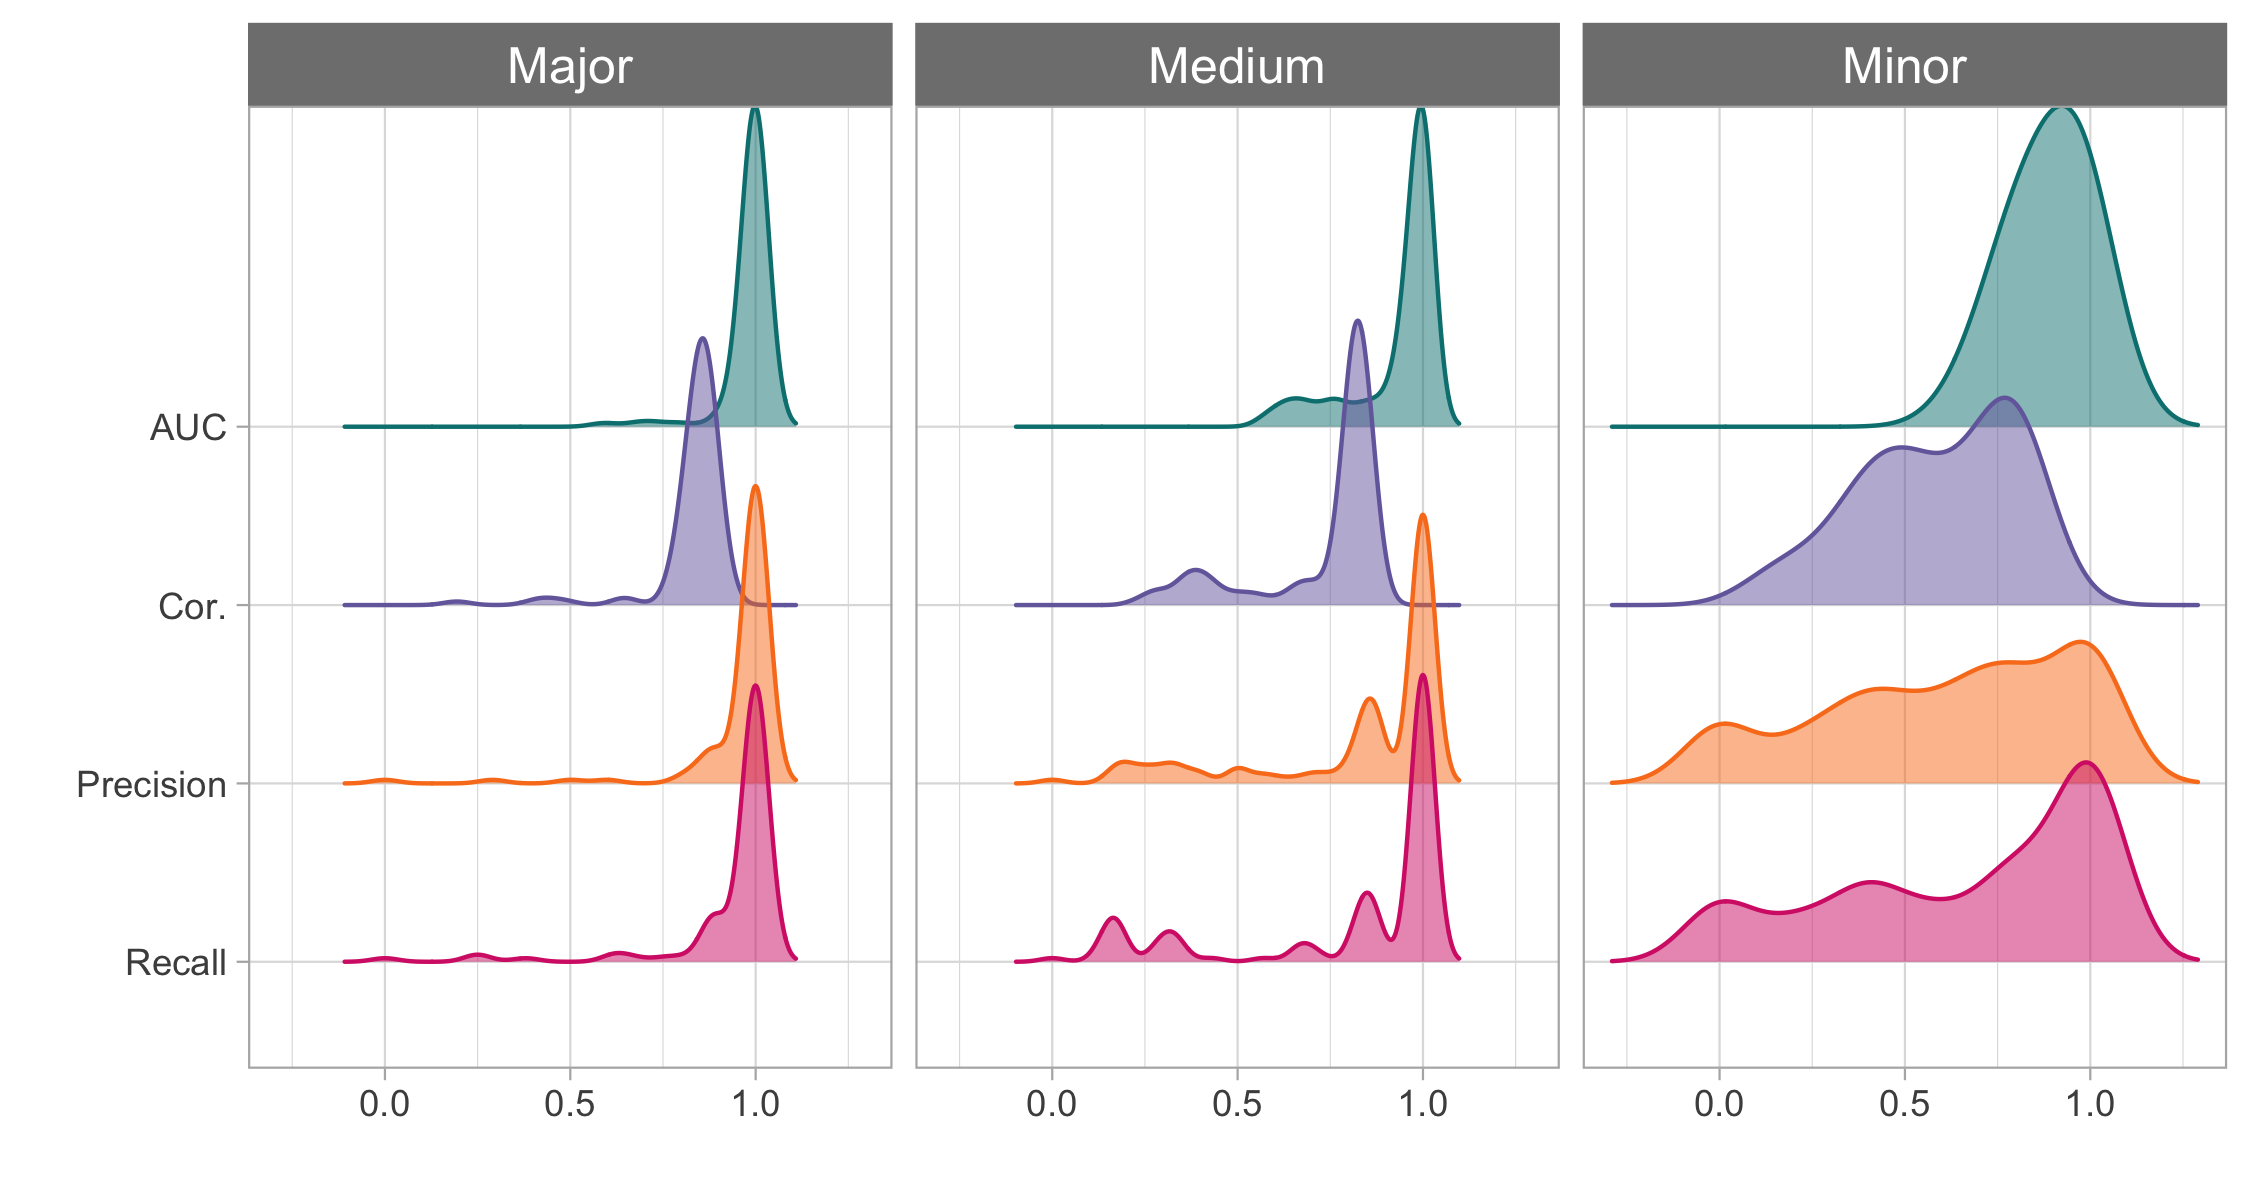
\includegraphics[width=11cm]{figs/simu_densities.png}
    \caption{
    %\CA{}
    The influence of the missing actor is measured with its degree, distinguishing three influence classes: \textit{Minor} (degree $\leq 5$), \textit{Medium} ($5<$ degree $\leq 7$) and \textit{Major} (degree $\geq 8$). 
    %\CA{Distributions of performance measures}
    The distributions of performance measures are displayed for each class of influence: AUC measures the retrieval of the dependence structure between all variables, observed and missing.  Precision and recall are specific to the missing actor links. 
    }
    \label{fig:densities}
\end{figure}
 

\begin{figure}[H]
    \centering    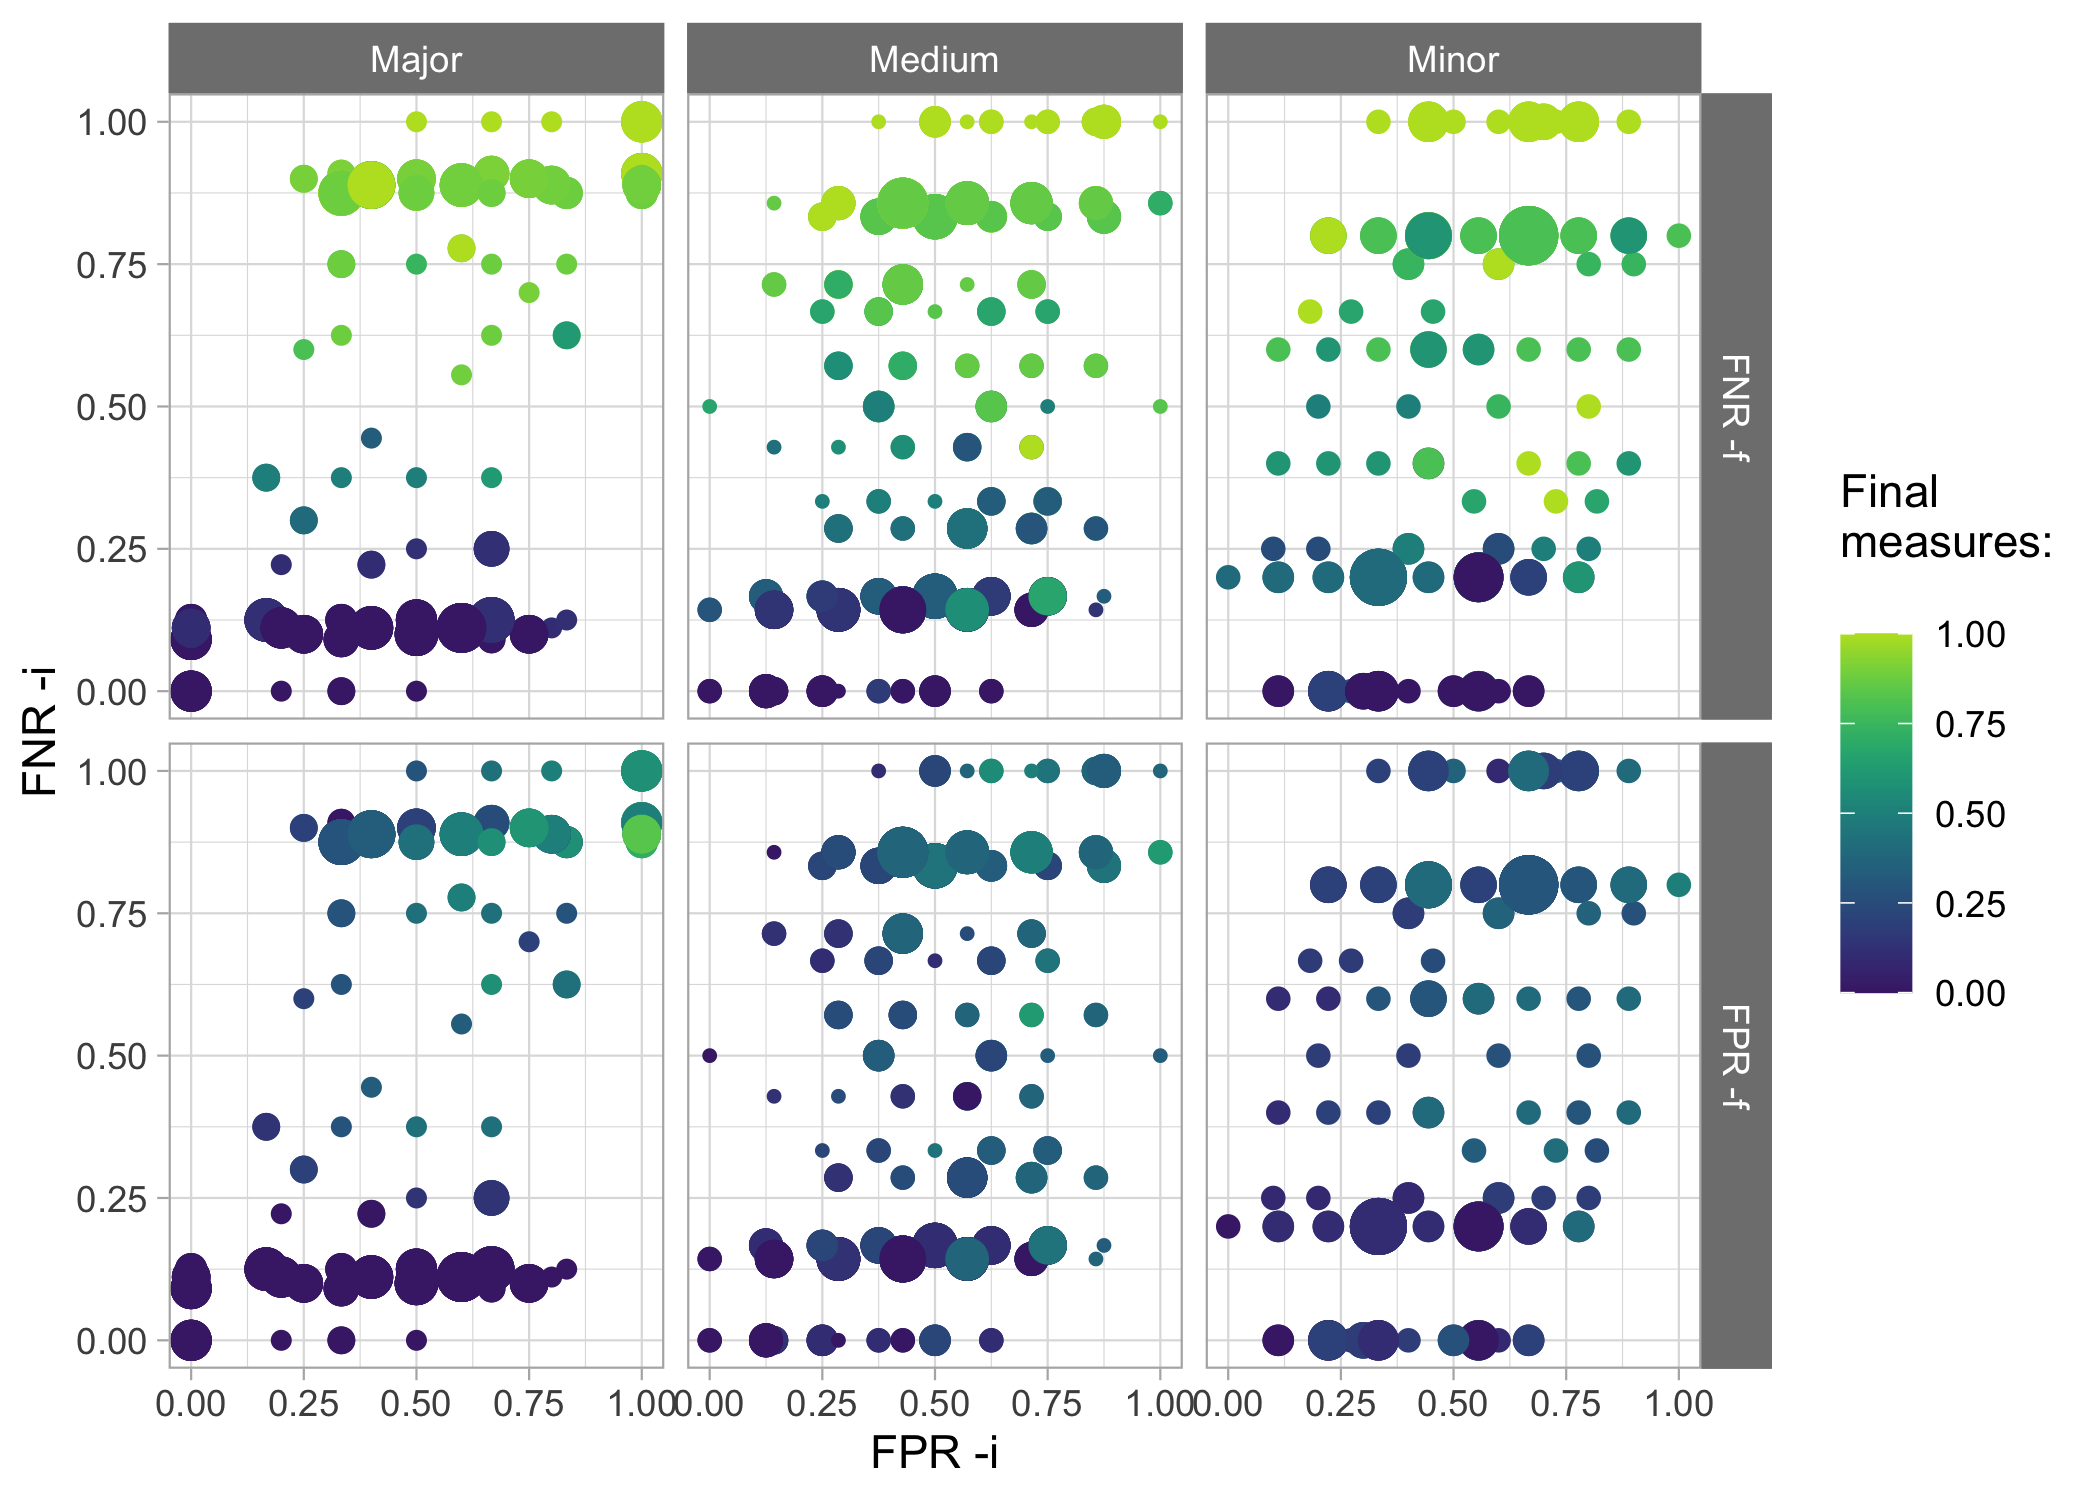
\includegraphics[width=11cm]{figs/quali_init_spca.png}
    \caption{Comparison of initial and final FPR and FNR, for cliques of neighbors of one missing actor obtained with the sparse PCA method. Position of dots are defined according to initial values, their color according to the final FPR and FNR. Sizes are proportional to the density of dots on a given position.}
    \label{fig:perfinit}
\end{figure}


 \begin{table}
\centering
\begin{tabular}{lrrrrrr}
  \hline
  & N & AUC & Precision & Recall & Cor. &t(s) \\ 
  \hline
  Major & 100 & 1 (0.00) & 1 (0.00) & 1 (0.01) & 0.86 (0.02)  & 1.28 (0.21) \\ 
  Medium & 132 & 1 (0.02) & 1 (0.00) & 0.99 (0.04) & 0.83 (0.02)  & 1.38 (0.46)  \\ 
  Minor &  68 & 0.98 (0.04) & 0.99 (0.03) & 0.96 (0.12) & 0.8 (0.04)& 1.56 (0.69) \\ 
   \hline
\end{tabular}
 \caption{\label{tab:oracle} Oracle procedure using true clique as starting point. The influence of the missing actor is measured with its degree, distinguishing three influence classes: \textit{Minor} (degree $\leq 5$), \textit{Medium} ($5<$ degree $\leq 7$) and \textit{Major} (degree $\geq 8$).  For each class of influence, the following quantities are reported:  number of simulated graphs (N), means and standard deviations of AUC, Precision, Recall, Correlation between missing actor inferred vector of means and original latent vector, and running times in seconds. AUC measures the retrieval of the dependence structure between all variables (observed and missing), whereas precision and recall are specific to the missing actor links.}
\end{table}